\section{Progettazione concettuale}
\subsection{Introduzione}
Il modello concettuale rappresenta la struttura logica del database, definendo le entità, gli attributi e le relazioni tra di esse. In questa fase, si è proceduto a identificare le principali entità del sistema e a stabilire le relazioni che le collegano, garantendo così una visione chiara e coerente delle informazioni da gestire.
\subsection{UML non ristrutturato}
\begin{figure}[H]
    \noindent\makebox[\linewidth]{%
        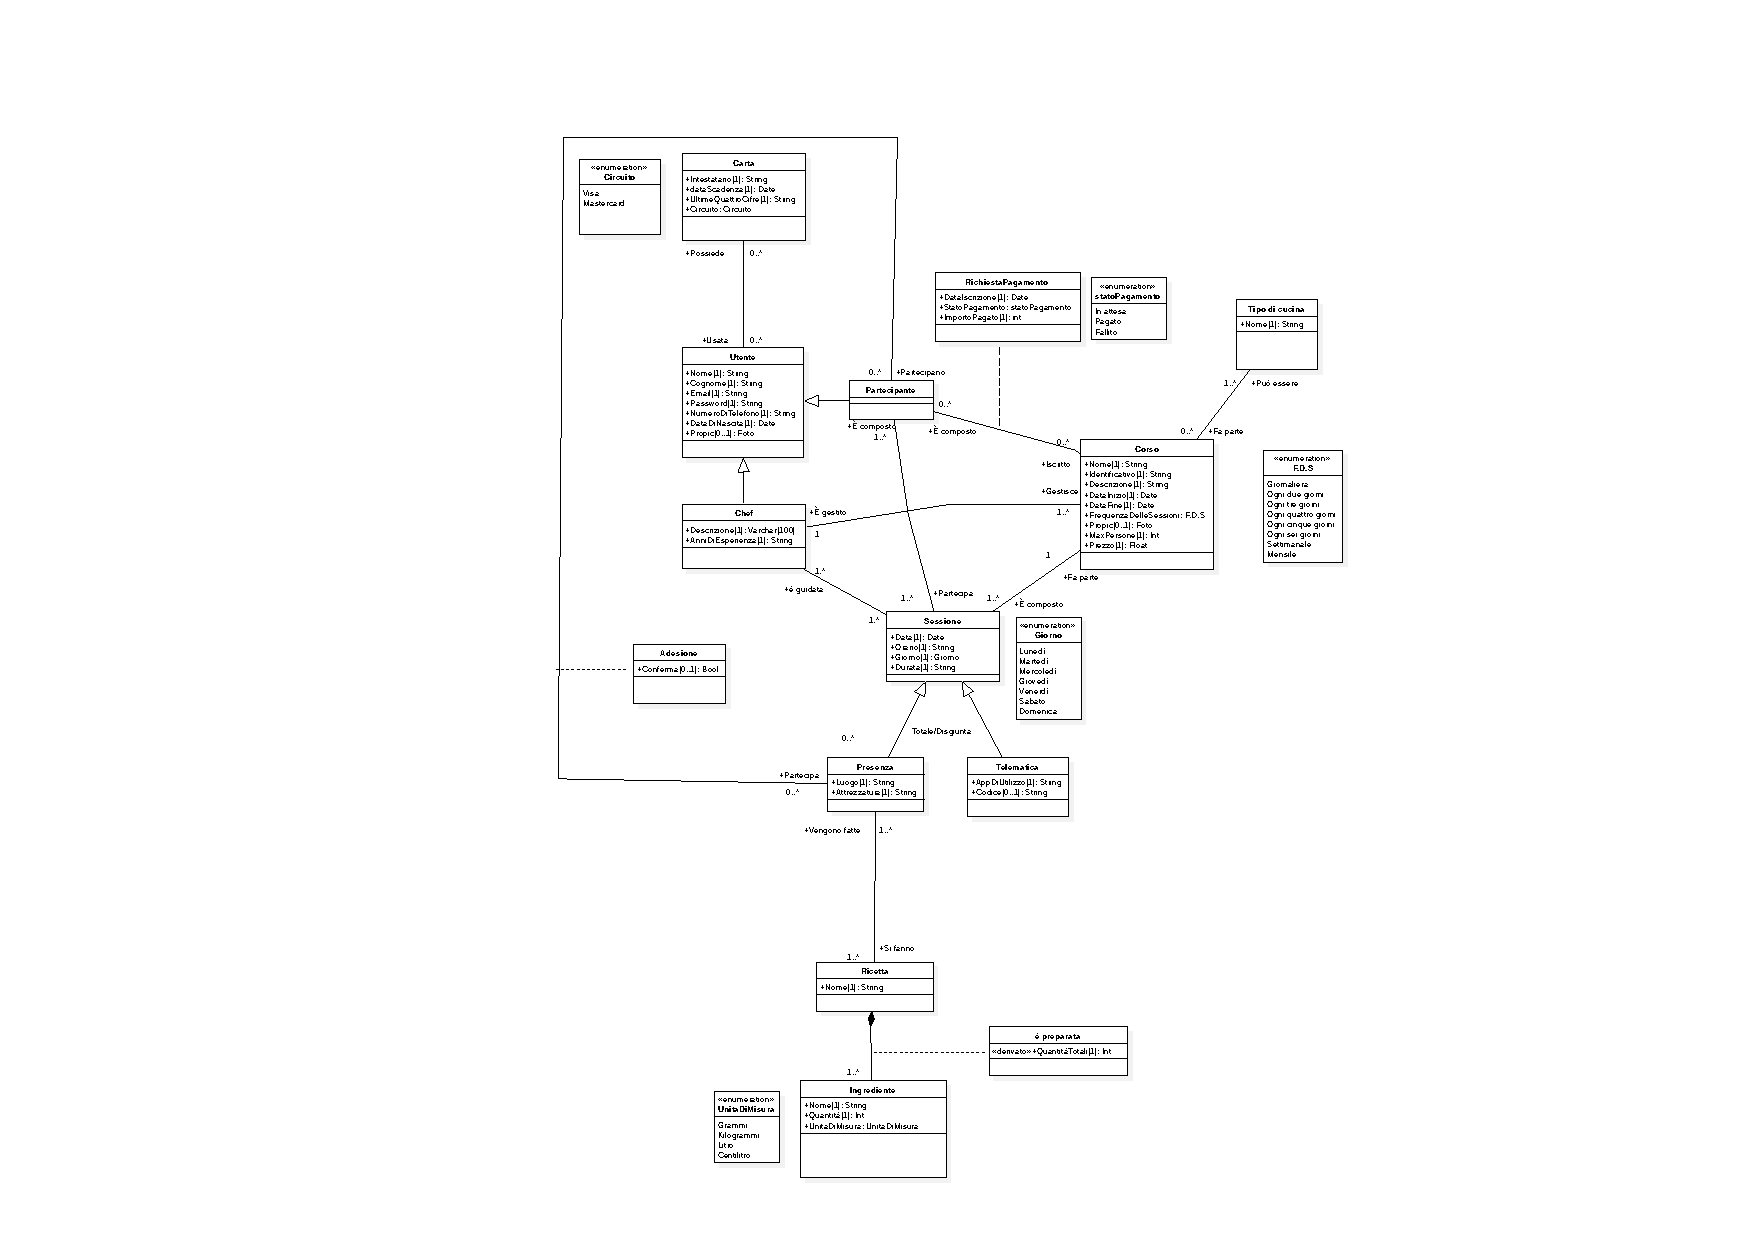
\includegraphics[height=0.9\textheight,width=2\textwidth]{latex/immagini/uml_non_ristrutturato.pdf}
    }
    \caption{Diagramma UML non ristrutturato}
\end{figure}
\subsubsection{Entità principali}
Le entità principali identificate nel sistema sono:
\begin{itemize}
    \item \textbf{Utente}: L’utente rappresenta il soggetto fruitore del sistema, che può iscriversi ai corsi e partecipare alle sessioni. I principali attributi includono nome, cognome, email, password, data di nascita e una foto di profilo. Ogni utente può essere associato a una o più carte di pagamento e può diventare partecipante a diversi corsi.
    \item \textbf{Chef}: Lo chef è un utente con il ruolo specifico di organizzare corsi. Ogni chef dispone di una descrizione e di un numero di anni di esperienza. Un chef può gestire più corsi, ma ogni corso è gestito da un solo chef.
    \item \textbf{Corso}: Il corso è l'entità centrale del sistema e rappresenta una proposta didattica su un tema gastronomico specifico. Contiene attributi quali nome, descrizione, identificativo, data di inizio/fine, frequenza delle sessioni, prezzo, massimo persone che possono iscriversi, immagine di copertina e tipo di cucina (gestito da un'altra entità). Ogni corso è composto da più sessioni e prevede una relazione molti-a-molti con i partecipanti.
    \item \textbf{Sessione}: Ogni corso è articolato in una o più sessioni, ciascuna delle quali ha una data, un orario, un insieme di giorni della settimana in cui si svolge, e una durata. Le sessioni sono specializzate in due sottotipi mutuamente esclusivi:
    \begin{itemize}
        \item \textbf{Presenza}: Con attributi come luogo e attrezzature richieste.
        \item \textbf{Telematica}: Con attributi relativi all'app utilizzata e al codice di accesso.
    \end{itemize}
    \item \textbf{Partecipante e Adesione}: La partecipazione ai corsi è modellata tramite l’entità Partecipante, che collega utenti e corsi. La partecipazione a sessioni pratiche richiede un’adesione esplicita, rappresentata dall'entità Adesione, che contiene un attributo booleano di conferma.
    \item \textbf{Ricetta e Ingredientemento}: Ogni sessione pratica può includere la preparazione di una o più ricette. Ogni ricetta è composta da uno o più ingredienti, ciascuno dei quali ha un nome, e un'unità di misura (enumerata). La relazione tra Ricetta e Ingrediente è associativa e include l'attributo QuantitàTotale e QuantitàUnitaria, utile per calcolare la quantità necessaria in base alle adesioni.
    \item \textbf{Carta e RichiestaPagamento}: I partecipanti  possono associare al proprio profilo una o più carte di pagamento, appartenenti a un circuito specificato tramite enumerazione (Visa, Mastercard). Le richieste di pagamento sono entità separate, con data, stato (in attesa, pagato, fallito) e importo.
\end{itemize}
\subsubsection{Gerarchie e generalizzazioni}
Nel modello concettuale, sono state identificate le seguenti gerarchie e generalizzazioni:
\begin{itemize}
    \item \textbf{Sessione}: Le sessioni sono suddivise in due sottotipi: \textit{Presenza} e \textit{Telematica}. Questa specializzazione consente di gestire le specificità di ciascun tipo di sessione, come il luogo e le attrezzature per le sessioni in presenza, e l'app utilizzata e il codice di accesso per quelle telematiche.
    \item \textbf{Utente}: L'entità Utente può essere specializzata in due sottotipi: \textit{Partecipante} e \textit{Chef}. Questa distinzione permette di gestire le diverse funzionalità e attributi associati a ciascun ruolo nel sistema.
\end{itemize}
Entrambe le specializzazioni sono totali e disgiunte, di conseguenza ogni istanza di Sessione sia esclusivamente di uno dei due tipi e che ogni Utente sia o un Partecipante o uno Chef, ma non entrambi contemporaneamente.
\subsubsection{Relazioni tra le entità}
Le relazioni tra le entità sono state definite come segue:
\begin{itemize}
    \item \textbf{Utente - Partecipante}: Un utente può essere un partecipante a più corsi, e ogni corso può avere più partecipanti. Questa relazione è molti-a-molti.
    \item \textbf{Chef - Corso}: Ogni chef può gestire più corsi, ma ogni corso è associato a un solo chef. Questa relazione è uno-a-molti.
    \item \textbf{Corso - Sessione}: Un corso può avere più sessioni, ma ogni sessione appartiene a un solo corso. Questa relazione è uno-a-molti.
    \item \textbf{Sessione - Partecipante}: Ogni partecipante può aderire a più sessioni pratiche, e ogni sessione può avere più partecipanti. Questa relazione è molti-a-molti, mediata dall'entità Adesione.
    \item \textbf{Corso - Ricetta}: Ogni corso può includere più ricette, e ogni ricetta può essere associata a più corsi. Questa relazione è molti-a-molti.
    \item \textbf{Ricetta - Ingrediente}: Ogni ricetta può includere più ingredienti, e ogni ingrediente può essere utilizzato in più ricette. Questa relazione è molti-a-molti, mediata dall'attributo QuantitàTotale.
    \item \textbf{Utente - Carta}: Un utente può avere più carte di pagamento associate al proprio profilo. Questa relazione è uno-a-molti.
    \item \textbf{Ricetta - Ingrediente}: Ogni ricetta può essere associata a più ingredienti, e ogni ingrediente può essere utilizzato in più ricette. Questa relazione è una composizione, mediata dall'attributo QuantitàTotale.
\end{itemize}
\subsubsection{Motivazione delle scelte progettuali}
Le scelte progettuali sono state guidate dalla necessità di garantire una rappresentazione chiara e coerente delle informazioni, facilitando la gestione dei corsi, delle sessioni e delle partecipazioni. La specializzazione delle sessioni in Presenza e Telematica consente di gestire le specificità di ciascun tipo di sessione, mentre la distinzione tra Partecipante e Chef permette di differenziare i ruoli degli utenti nel sistema. Inoltre, l'uso di relazioni molti-a-molti per gestire le adesioni alle sessioni pratiche e le associazioni tra ricette e ingredienti garantisce flessibilità e scalabilità nel modello.
\subsubsection{Diagramma ER}
Il diagramma ER (Entity-Relationship) rappresenta graficamente le entità principali del sistema, i loro attributi e le relazioni tra di esse, fornendo una visione sintetica e formale della struttura informativa del database.

\begin{figure}[H]
    \noindent\makebox[\linewidth]{%
        
\includegraphics[page=2, height=0.8\textheight, width=1\textwidth]{latex/immagini/ER.pdf}
    }
    \caption{Diagramma ER del sistema}
\end{figure}
\subsection{UML ristrutturato}
\begin{figure}[H]
    \noindent\makebox[\linewidth]{%
        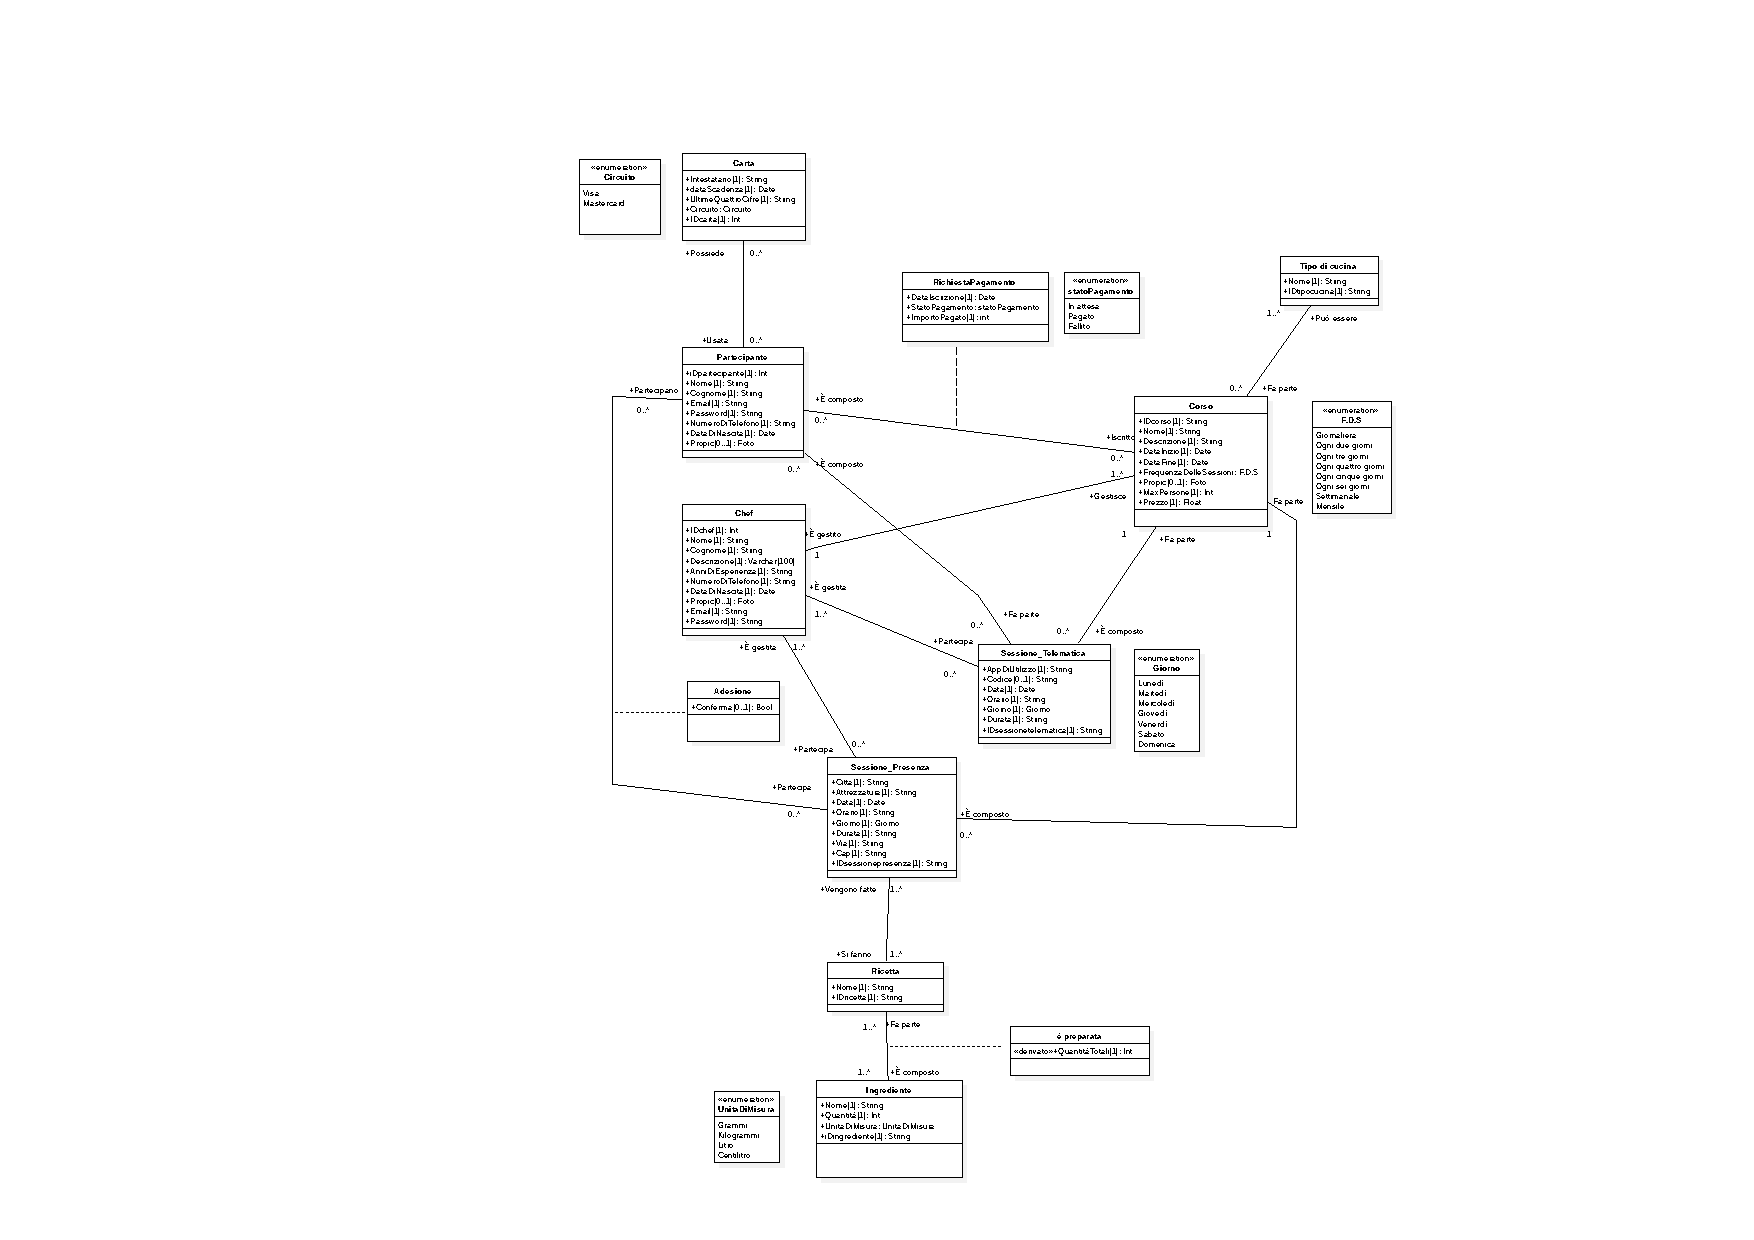
\includegraphics[height=0.9\textheight,width=2\textwidth]{latex/immagini/uml_ristrutturato.pdf}
    }
    \caption{Diagramma UML ristrutturato del sistema}
\end{figure}
\subsubsection{Modifiche rispetto al modello non ristrutturato}
Il modello ristrutturato presenta alcune modifiche rispetto al modello non ristrutturato, adattandolo a un database relazionale. Le principali modifiche includono:
\begin{itemize}
    \item \textbf{Rimozione delle gerarchie}: Le gerarchie tra le entità sono state rimosse, trasformando le specializzazioni in entità separate. Ad esempio, le sessioni di tipo Presenza e Telematica sono state trasformate in due entità distinte, mantenendo gli attributi specifici per ciascun tipo.
    \item \textbf{Attributi composti e multivalore}: Gli attributi composti e multivalore sono stati normalizzati. Ad esempio, l'attributo \textit{Luogo} è stato suddiviso in attributi separati per \textit{Città}, \textit{Indirizzo} e \textit{Cap}.
    \item \textbf{Aggiunta di chiavi primarie e esterne}: Ogni entità ha una chiave primaria univoca, e le relazioni tra le entità sono definite tramite chiavi esterne, garantendo l'integrità referenziale del database.
\end{itemize}

\subsubsection{Comportamento del modello ristrutturato con le modifiche}
Il modello ristrutturato mantiene le proprietà di specializzazione totale e disgiunta, adattandosi alle modifiche apportate. In particolare:
\begin{itemize}
    \item \textbf{Specializzazione totale e disgiunta}: Le entità separate per le sessioni di tipo Presenza e Telematica garantiscono che ogni sessione appartenga esclusivamente a uno dei due tipi, rispettando la disgiunzione. Inoltre, ogni utente è classificato come Partecipante o Chef, assicurando che la specializzazione sia totale e disgiunta.
    \item \textbf{Integrità referenziale}: L'uso di chiavi primarie, esterne e l'aggiunta di chiavi surrogate garantisce che le relazioni tra le entità siano coerenti e che non si verifichino violazioni di integrità nel database.
\end{itemize}

\subsubsection{Motivazioni delle scelte del modello ristrutturato}
Le motivazioni alla base delle scelte progettuali del modello ristrutturato derivano dalla necessità di garantire una rappresentazione chiara, coerente e scalabile delle informazioni, adattandosi alle esigenze di un database relazionale. Una delle principali considerazioni riguarda la gestione delle specializzazioni totali e disgiunte, che hanno permesso di semplificare il modello concettuale senza perdere la coerenza logica.

Nel modello ristrutturato, le specializzazioni totali e disgiunte sono state gestite trasformando la classe generale in entità separate per ciascuna specializzazione. Questo approccio consente di incorporare gli attributi della classe generale direttamente nelle entità specializzate, eliminando la necessità di mantenere una gerarchia tra le entità. Ad esempio, nel caso delle sessioni, la classe generale "\textbf{Sessione}" è stata suddivisa in due entità distinte: "\textbf{Sessione\_Presenza}" e "\textbf{Sessione\_Telematica}". Ogni entità specializzata include gli attributi specifici del proprio tipo, come il luogo e le attrezzature richieste per le sessioni in presenza, e l'app utilizzata e il codice di accesso per quelle telematiche. In questo modo, si garantisce che ogni sessione appartenga esclusivamente a uno dei due tipi, rispettando la disgiunzione, e che tutte le sessioni siano rappresentate nel modello, rispettando la totalità, facilitando anche le associazioni tra le varie entità.

La stessa logica è stata applicata alla specializzazione dell'entità "Utente", suddivisa in "Partecipante" e "Chef". Ogni utente è classificato come Partecipante o Chef, ma non può appartenere a entrambe le categorie contemporaneamente. Gli attributi comuni agli utenti, come nome, cognome, email e data di nascita, sono stati incorporati direttamente nelle entità specializzate, mentre gli attributi specifici, come la descrizione e gli anni di esperienza per gli Chef, sono stati aggiunti solo alla rispettiva entità. Questo approccio semplifica la gestione delle entità nel database, eliminando la necessità di un'entità generale "Utente" e garantendo che la specializzazione rimanga totale e disgiunta.

Per quanto riguarda le associazioni tra le entità, il modello ristrutturato utilizza chiavi primarie e chiavi esterne per definire le relazioni, garantendo l'integrità referenziale del database. Ad esempio, la relazione tra "Corso" e "Sessione" è uno-a-molti, con l'identificativo del corso utilizzato come chiave esterna nelle entità "Presenza" e "Telematica". Questo approccio consente di mantenere la coerenza delle informazioni e di semplificare le operazioni di query e aggiornamento. Analogamente, la relazione molti-a-molti tra "Sessione" e "Partecipante" è mediata dall'entità "Adesione", che include un attributo booleano di conferma per gestire la partecipazione alle sessioni pratiche.

Un altro esempio significativo riguarda la relazione tra "Ricetta" e "Ingrediente". Nel modello ristrutturato, questa relazione è stata normalizzata utilizzando un'entità associativa che include l'attributo "QuantitàTotale". Questo approccio consente di calcolare facilmente la quantità necessaria di ciascun ingrediente in base alle adesioni alle sessioni pratiche, garantendo flessibilità e scalabilità nel modello.
\begin{figure}[H]
    \noindent\makebox[\linewidth]{
        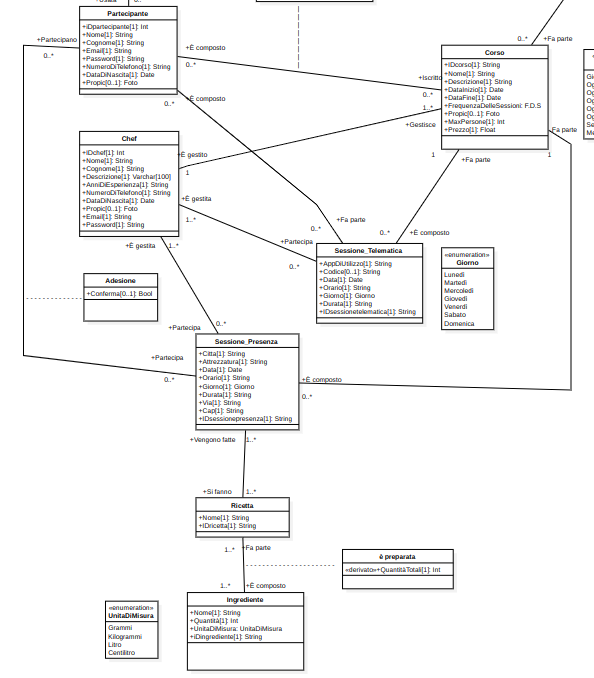
\includegraphics[height=0.8\textheight,width=1\textwidth]{latex/immagini/uml_ristrutturato_sessioni.png}
    }
    \caption{Scelte ristrutturato}
\end{figure}

\subsection{Dizionari}

\subsubsection{Dizionario delle Classi (Entità)}

\paragraph{Entità Principali - Parte 1}

\begin{center}
\begin{tcolorbox}[colback=white!98!gray, colframe=myblue!80!black, title=Dizionario delle Classi (Entità) - Parte 1, arc=4mm, boxrule=0.8pt, width=0.98\textwidth]
\renewcommand{\arraystretch}{1.2}
\begin{tabularx}{\textwidth}{p{3.2cm}p{4.8cm}X}
\textbf{Classe} & \textbf{Descrizione} & \textbf{Attributi} \\
\hline
CARTA & Rappresenta una carta di pagamento associata a un partecipante. & IdCarta (PK), Intestatario, DataScadenza, UltimeQuattroCifre, Circuito \\
\hline
PARTECI\-PANTE & Utente che si iscrive e partecipa ai corsi di cucina. & IdPartecipante (PK), Nome, Cognome, Email, Password, DataDiNascita, Propic \\
\hline
POSSIEDE & Entità associativa che rappresenta il possesso di carte di pagamento da parte dei partecipanti. & IdPartecipante (FK, PK), IdCarta (FK, PK) \\
\hline
CHEF & Utente specializzato nell'organizzazione e gestione dei corsi di cucina. & IdChef (PK), Nome, Cognome, Email, Password, DataDiNascita, Descrizione, Propic, AnniDiEsperienza \\
\hline
CORSO & Rappresenta un corso di cucina tematico con tutte le sue caratteristiche. & IdCorso (PK), Nome, Descrizione, DataInizio, DataFine, FrequenzaDelleSessioni, Propic, MaxPersone, Prezzo, IdChef (FK) \\
\hline
RICHIESTA\-PAGAMENTO & Gestisce le richieste di pagamento per l'iscrizione ai corsi. & DataRichiesta, StatoPagamento, ImportoPagato, IdCorso (FK), IdPartecipante (FK) \\
\hline
TIPODICUCINA & Definisce le tipologie di cucina disponibili per i corsi. & IDTipoCucina (PK), Nome \\
\hline
TIPODICUCINA\_\-CORSO & Entità associativa che collega i corsi alle tipologie di cucina. & IDTipoCucina (FK, PK), IDCorso (FK, PK) \\
\hline
\end{tabularx}
\end{tcolorbox}
\end{center}

\paragraph{Entità Principali - Parte 2}

\begin{center}
\begin{tcolorbox}[colback=white!98!gray, colframe=myblue!80!black, title=Dizionario delle Classi (Entità) - Parte 2, arc=4mm, boxrule=0.8pt, width=0.98\textwidth]
\renewcommand{\arraystretch}{1.2}
\begin{tabularx}{\textwidth}{p{3.2cm}p{4.8cm}X}
\textbf{Classe} & \textbf{Descrizione} & \textbf{Attributi} \\
\hline
SESSIONE\_\-PRESENZA & Rappresenta una sessione di corso che si svolge fisicamente in presenza. & IdSessionePresenza (PK), Giorno, Data, Orario, Durata, Citta, Via, Cap, Attrezzatura, Descrizione, IDCorso (FK), IDChef (FK) \\
\hline
SESSIONE\_\-TELEMATICA & Rappresenta una sessione di corso che si svolge online in modalità telematica. & IdSessioneTelematica (PK), Applicazione, CodiceChiamata, Data, Orario, Durata, Giorno, Descrizione, IDCorso (FK), IdChef (FK) \\
\hline
PARTECIPANTE\_\-SESSIONETE\-LEMATICA & Entità associativa per la partecipazione alle sessioni telematiche. & IdPartecipante (FK, PK), IdSessioneTelematica (FK, PK) \\
\hline
ADESIONE\_\-SESSIONEPRE\-SENZA & Gestisce l'adesione dei partecipanti alle sessioni in presenza. & Conferma, IdSessionePresenza (FK, PK), IDPartecipante (FK, PK) \\
\hline
RICETTA & Rappresenta una ricetta culinaria utilizzata durante le sessioni. & IdRicetta (PK), Nome \\
\hline
SESSIONE\_\-PRESENZA\_\-RICETTA & Entità associativa che collega le sessioni in presenza alle ricette utilizzate. & IdRicetta (FK, PK), IdSessionePresenza (FK, PK) \\
\hline
INGREDIENTE & Rappresenta un ingrediente utilizzato nelle ricette. & IdIngrediente (PK), Nome, UnitaDiMisura \\
\hline
PREPARAZIONE\-INGREDIENTE & Entità associativa che definisce gli ingredienti necessari per ogni ricetta con le relative quantità. & IdRicetta (FK, PK), IdIngrediente (FK, PK), QuantitaTotale, QuantitaUnitaria \\
\hline
\end{tabularx}
\end{tcolorbox}
\end{center}



\subsubsection{Dizionario delle Associazioni (Relazioni) - Parte 1}
\begin{center}
\begin{tcolorbox}[colback=white!98!gray, colframe=myblue!80!black, title=Dizionario delle Associazioni (Relazioni) - Parte 1, arc=4mm, boxrule=0.8pt, width=0.98\textwidth]
\renewcommand{\arraystretch}{1.2}
\begin{tabularx}{\textwidth}{p{3.8cm}p{4.2cm}X}
\textbf{Associazione} & \textbf{Descrizione} & \textbf{Classi coinvolte} \\
\hline
POSSIEDE & Relazione molti-a-molti che consente ai partecipanti di possedere multiple carte di pagamento. & \textbf{PARTECIPANTE} (0..n) $\leftrightarrow$ \textbf{CARTA} (0..n) \\
\hline
CORSO - CHEF & Relazione uno-a-molti: ogni corso è gestito da un solo chef, ma ogni chef può gestire più corsi contemporaneamente. & \textbf{CORSO} (0..n) $\rightarrow$ \textbf{CHEF} (1) \\
\hline
CORSO - TIPODICUCINA & Relazione molti-a-molti implementata tramite l'entità associativa TIPODICUCINA\_\-CORSO per gestire corsi con multiple tipologie. & \textbf{CORSO} (0..n) $\leftrightarrow$ \textbf{TIPODICUCINA} (0..n) \\
\hline
CORSO - SESSIONI & Relazione uno-a-molti: ogni corso può avere multiple sessioni (sia in presenza che telematiche). & \textbf{CORSO} (1) $\rightarrow$ \textbf{SESSIONE\_\-PRESENZA} (0..n), \textbf{SESSIONE\_\-TELEMATICA} (0..n) \\
\hline
SESSIONE\_\-PRESENZA - PARTECIPANTI & Relazione molti-a-molti tramite ADESIONE\_\-SESSIONEPRE\-SENZA per gestire la partecipazione alle sessioni in presenza. & \textbf{SESSIONE\_\-PRESENZA} (0..n) $\leftrightarrow$ \textbf{PARTECIPANTE} (0..n) \\
\hline
\end{tabularx}
\end{tcolorbox}
\end{center}


\subsubsection{Dizionario delle Associazioni (Relazioni) - Parte 2}
\begin{center}
\begin{tcolorbox}[colback=white!98!gray, colframe=myblue!80!black, title=Dizionario delle Associazioni (Relazioni) - Parte 2, arc=4mm, boxrule=0.8pt, width=0.98\textwidth]
\renewcommand{\arraystretch}{1.2}
\begin{tabularx}{\textwidth}{p{3.8cm}p{4.2cm}X}
\textbf{Associazione} & \textbf{Descrizione} & \textbf{Classi coinvolte} \\
\hline
SESSIONE\_TELEMATICA\- - PARTECI\-PANTI & Relazione molti-a-molti tramite PARTECIPANTE\_\-SESSIONETE\-LEMATICA per gestire la partecipazione alle sessioni online. & \textbf{SESSIONE\_\-TELEMATICA} (0..n) $\leftrightarrow$ \textbf{PARTECIPANTE} (0..n) \\
\hline
SESSIONE\_\-PRESENZA - RICETTE & Relazione molti-a-molti tramite SESSIONE\_\-PRESENZA\_\-RICETTA per associare ricette alle sessioni pratiche. & \textbf{SESSIONE\_\-PRESENZA} (0..n) $\leftrightarrow$ \textbf{RICETTA} (0..n) \\
\hline
RICETTA - INGREDIENTI & Relazione molti-a-molti tramite PREPARAZIONE\-INGREDIENTE per definire gli ingredienti necessari per ogni ricetta. & \textbf{RICETTA} (0..n) $\leftrightarrow$ \textbf{INGREDIENTE} (0..n) \\
\hline
RICHIESTA\-PAGAMENTO & Relazione molti-a-uno che collega ogni richiesta di pagamento a un partecipante e a un corso specifico. & \textbf{PARTECIPANTE} (0..n), \textbf{CORSO} (1) $\rightarrow$ \textbf{RICHIESTAPAGAMENTO} \\
\hline
\end{tabularx}
\end{tcolorbox}
\end{center}

\subsubsection{Dizionario dei vincoli }

\paragraph{Vincoli di Dominio}

\begin{center}
\begin{tcolorbox}[colback=white!98!gray, colframe=myblue!80!black, title=Vincoli di Dominio, arc=4mm, boxrule=0.8pt, width=0.98\textwidth]
\renewcommand{\arraystretch}{1.2}
\begin{tabularx}{\textwidth}{p{4cm}X}
\textbf{Attributo} & \textbf{Dominio e Vincoli} \\
\hline
\textbf{StatoPagamento} & $\in$ \{``In Attesa'', ``Pagato'', ``Fallito''\}. Rappresenta lo stato attuale di una transazione di pagamento. \\
\hline
\textbf{Circuito} & $\in$ \{``Visa'', ``Mastercard''\}. Definisce il circuito della carta di pagamento utilizzata. \\
\hline
\textbf{Email} & Deve rispettare il formato (es. utente@dominio.com). Garantisce la validità dell'indirizzo email per le comunicazioni. \\
\hline
\textbf{MaxPersone} & Intero positivo $> 0$. Definisce la capacità massima di partecipanti per corso. \\
\hline
\textbf{Prezzo} & Decimale $\geq 0.00$ con precisione di 2 cifre decimali. Rappresenta il costo del corso in Euro. \\
\hline
\textbf{Durata} & Intero positivo espresso in minuti, $> 0$ e $\leq 480$ (8 ore). Definisce la durata di una sessione. \\
\hline
\textbf{Età} & Data di nascita deve corrispondere a età compresa tra 18 e 100 anni. Validata tramite trigger per garantire utenti maggiorenni. \\
\hline
\textbf{TipoCucina} & Massimo 2 tipi di cucina diversi per corso. Implementato tramite trigger per limitare la varietà culinaria per corso. \\
\hline
\end{tabularx}
\end{tcolorbox}
\end{center}

\paragraph{Vincoli Intra-relazionali}

\begin{center}
\begin{tcolorbox}[colback=white!98!gray, colframe=myblue!80!black, title=Vincoli Intra-relazionali, arc=4mm, boxrule=0.8pt, width=0.98\textwidth]
\renewcommand{\arraystretch}{1.2}
\begin{tabularx}{\textwidth}{p{4cm}X}
\textbf{Vincolo} & \textbf{Descrizione e Applicazione} \\
\hline
\textbf{Chiavi Primarie} & Ogni entità ha una chiave primaria univoca seguendo la convenzione IdNomeEntità (es. IdUtente, IdCorso). Garantisce identificazione univoca di ogni istanza. \\
\hline
\textbf{Vincoli NOT NULL} & Attributi obbligatori non possono essere nulli: tutte le chiavi primarie, attributi Nome, Email degli utenti, DataInizio/DataFine dei corsi, Titolo delle ricette. \\
\hline
\textbf{Vincoli di Unicità} & Email in UTENTE deve essere univoca nel sistema sia per chef che partecipante e tra loro . \\
\hline
\textbf{Vincoli CHECK} & DataInizio $<$ DataFine in CORSO. \\
\hline
\textbf{Vincoli via Trigger} & Implementati vari trigger specifici per vincoli complessi (dettagliati nel Cap. 4.2): limite 2 tipi cucina per corso, controllo pagamenti, gestione modifiche corsi non iniziati, controllo adesioni solo per iscritti. \\
\hline
\end{tabularx}
\end{tcolorbox}
\end{center}

\paragraph{Vincoli Inter-relazionali}

\begin{center}
\begin{tcolorbox}[colback=white!98!gray, colframe=myblue!80!black, title=Vincoli Inter-relazionali, arc=4mm, boxrule=0.8pt, width=0.98\textwidth]
\renewcommand{\arraystretch}{1.2}
\begin{tabularx}{\textwidth}{p{4cm}X}
\textbf{Vincolo} & \textbf{Descrizione e Applicazione} \\
\hline
\textbf{Integrità Referenziale} & Tutte le chiavi esterne devono riferirsi a valori esistenti nelle tabelle padre. Implementata tramite FOREIGN KEY con CASCADE/RESTRICT appropriati. \\
\hline
\textbf{Specializzazione UTENTE} & Ogni UTENTE deve essere esattamente uno tra CHEF o PARTECIPANTE (specializzazione totale e disgiunta). Implementata tramite vincoli CHECK o trigger. \\
\hline
\textbf{Specializzazione SESSIONE} & Ogni SESSIONE deve essere esattamente una tra SESSIONE\_PRESENZA o SESSIONE\_TELEMATICA (specializzazione totale e disgiunta). \\
\hline
\textbf{Vincoli di Cardinalità} & Un CORSO deve avere almeno 1 SESSIONE. Un PARTECIPANTE può avere 0..n CARTE. Una RICETTA deve avere almeno 1 INGREDIENTE (tramite PREPARAZIONEINGREDIENTE). \\
\hline
\textbf{Vincoli di Capacità} & Il numero di iscrizioni per un CORSO non può superare MaxPersone del corso stesso. Il numero di carte per PARTECIPANTE è limitato (max 5). Impedimento eliminazione corsi con iscritti paganti. Implementati tramite trigger specifici. \\
\hline
\textbf{Vincoli Temporali} & Le SESSIONI di un CORSO devono avere Data compresa tra DataInizio e DataFine del corso. DataPagamento in RICHIESTAPAGAMENTO $\leq$ DataInizio del corso associato. Controllo orario e durata sessioni. Impedimento modifiche/disiscrizioni dopo inizio corso. Validazione corrispondenza importo pagato con costo corso. \\
\hline
\textbf{Vincoli di Conflitto} & Un CHEF non può essere assegnato contemporaneamente a sessioni di presenza e telematiche nello stesso orario. Un PARTECIPANTE può aderire solo a sessioni di corsi a cui è iscritto. Eliminazione automatica ingredienti quando viene eliminata la ricetta associata. \\
\hline
\end{tabularx}
\end{tcolorbox}
\end{center}

\paragraph{Vincoli di Molteplicità (n-plu)}

\begin{center}
\begin{tcolorbox}[colback=white!98!gray, colframe=myblue!80!black, title=Vincoli di Molteplicità, arc=4mm, boxrule=0.8pt, width=0.98\textwidth]
\renewcommand{\arraystretch}{1.2}
\begin{tabularx}{\textwidth}{p{5cm}X}
\textbf{Relazione} & \textbf{Cardinalità e Vincoli} \\
\hline
\textbf{CHEF - CORSO} & (1,n) : (1,1) - Ogni chef può creare più corsi, ogni corso è creato da un unico chef. \\
\hline
\textbf{PARTECIPANTE - ADESIONE} & (1,1) : (0,n) - Ogni adesione è di un partecipante, ogni partecipante può avere più adesioni. \\
\hline
\textbf{CORSO - ADESIONE} & (1,1) : (0,n) - Ogni adesione è per un corso, ogni corso può avere più adesioni (max MaxPersone). \\
\hline
\textbf{PARTECIPANTE - CARTA} & (1,1) : (0,n) - Ogni carta appartiene a un partecipante, ogni partecipante può avere più carte (max 5). \\
\hline
\textbf{RICETTA - INGREDIENTE} & (n,n) tramite PREPARAZIONEINGREDIENTE - Una ricetta usa più ingredienti, un ingrediente può essere in più ricette. \\
\hline
\textbf{SESSIONE\_PRESENZA - RICETTA} & (n,n) tramite SESSIONE\_PRESENZA\_RICETTA - Una sessione può usare più ricette, una ricetta può essere usata in più sessioni. \\
\hline
\end{tabularx}
\end{tcolorbox}
\end{center}



